\chapter{公平性}
\label{chap:trust-fairness}

培训名额模型总体预测准确，却可能集中拒绝某一群体的合格者。我们要评价这个后果，既需看错误落在哪些人身上，也需先确定名额应怎样分配。各组准确率相同，仍可能有不同误拒、误收、机会数量和实际损失。

前两章已经提供了错误和环境条件的证据，还没有给出人之间的分配原则。预测可靠或稳定不能决定机会、负担怎样才合理，公平性需要在这些证据之上声明自己的要求。

在第~\ref{chap:trust-foundations}章的三层框架中，公平要求先确定比较哪些待遇、错误和影响路径；群体统计、个体对照、因果分析与内容评价再提供证据。群体构成、标签产生和长期后果改变时，还需监测、复查与纠正，使结论在生命周期中保持限定范围。

本章以名额分配研究保护对象、判定证据和干预。先从具体待遇及形成原因建立比较对象，再把保护维度转为准则与检验，最后定位数据、训练、决策中的修改。准则决定要改善什么，机制决定改哪里，即时效果和长期反馈再检验措施是否真正改善后果。

图~\ref{fig:trust-fairness-opportunity}固定两人的认可资格。教学设定假定三个项目已经覆盖全部分配依据，也没有许可的抽签机制；若无关差异稳定地产生不同待遇，就违反这一场景的个体一致性。现实审计还需验证资格充分和随机机制等条件，材料看似相近本身不够。

\begin{figure*}[!htb]
  \centering
  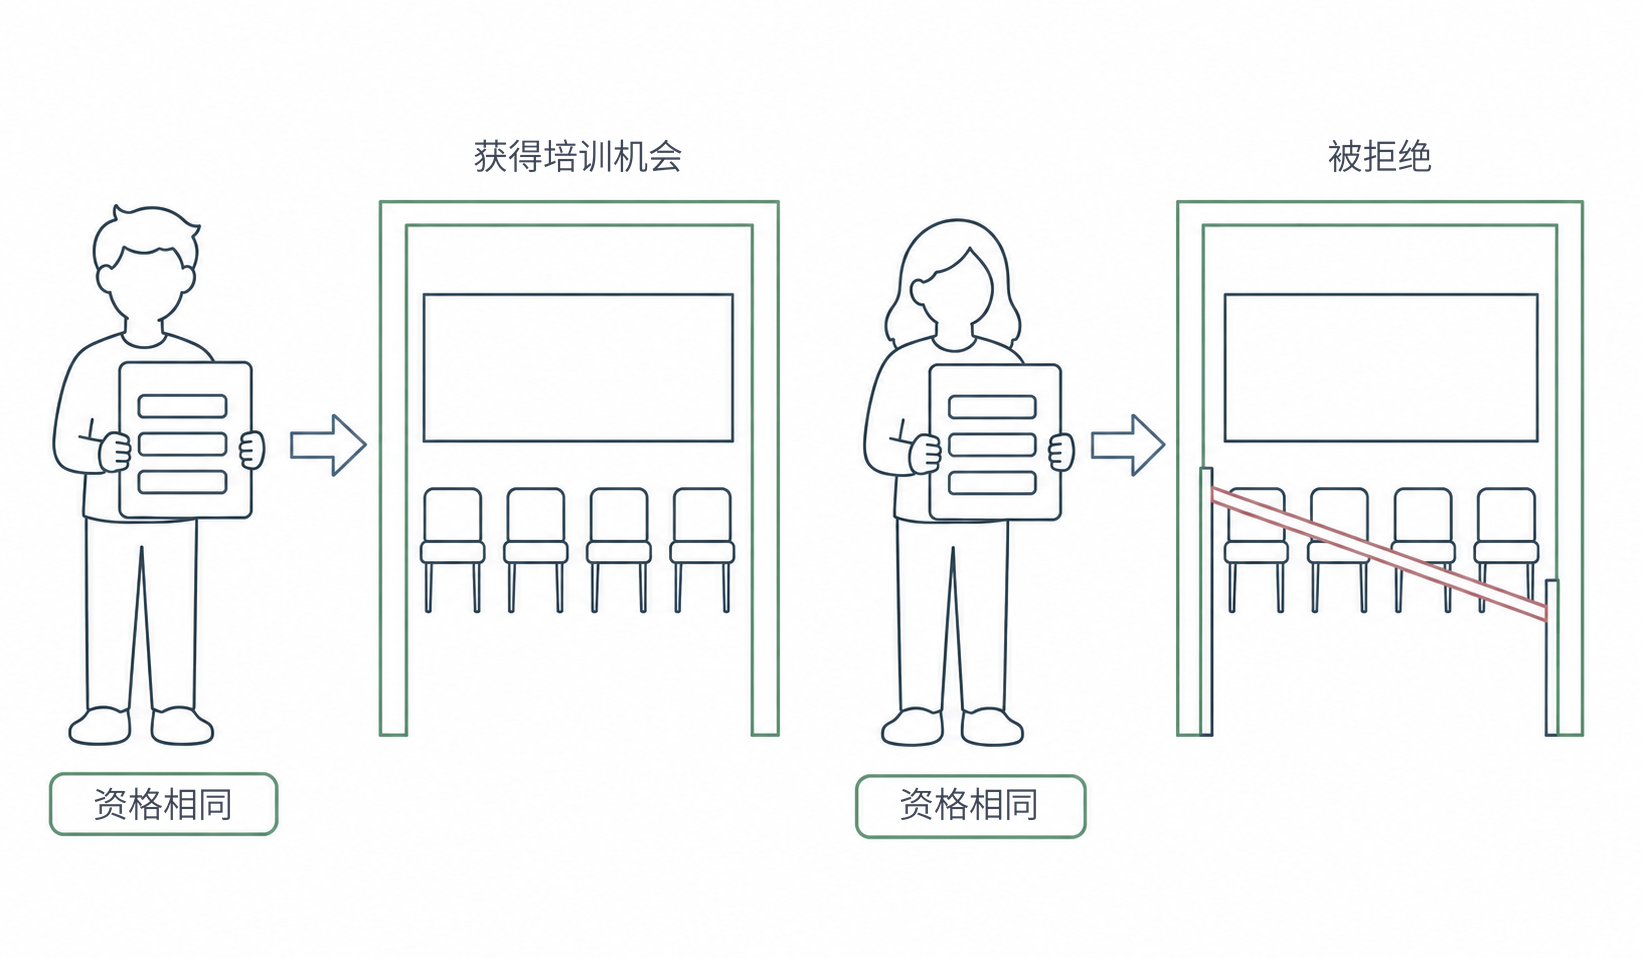
\includegraphics[width=132.000mm]{figures/03-foundations/03-trustworthiness/generated/fairness-opportunity/figure.png}
  \caption{同一系统处理两个认可资格相同的申请者，三个相同图标示意资格，一人获选、一人被拒，提示调查个体差别。人物外观只区别对象，未指定差异原因。图为构造情景。}
  \label{fig:trust-fairness-opportunity}
\end{figure*}

\section{模型的公平性}
\label{sec:fairness-concepts}

\subsection{公平性的含义}
\label{sec:fairness-meaning}

\term{公平性}（fairness）依据任务认可的原则，评价模型与流程怎样在不同人之间分配机会、收益、错误和负担。除了谁获得什么，还需检查决定依据及纠正待遇的途径。适用同一准则，并不要求所有人的输出都相同，必须先说明哪些差异合理，哪些违背保护要求。

现有资格、培训预期收益和弥补机会不足，是三种可能的名额原则，可能产生不同名单。准确率无法选出唯一合理原则。规范判断先确定允许和应纠正的差异，统计方法随后检查要求，二者职责不同。

为把资格与机会分开，记可用非群体特征$\bm{x}$、关注属性$a$、资格标签$y\in\{0,1\}$及决策$\hat y$。部署读取$a$时，合格概率分数为$S=p(\bm{x},a)$，否则为$S=p(\bm{x})$；决策分布相应记$q_{\bm{x},a}$或$q_{\bm{x}}$，确定性决策是退化分布。审计仍可按$a$分组，不等于预测使用$a$。培训例中$y=1$为按认可标准合格，$\hat y=1$为获选，历史录取不能直接充当资格。邮件的正决策表示隔离，此处表示机会，错误方向必须随含义解释。

样本人数、预测分数、录取决定、参加成本和最终收益属于不同环节。同概率经不同阈值可获得不同机会，同机会经不同费用与服务可得到不同收益。系统边界需包含这些环节，局部均等尚未评价完整后果。

\subsection{不公平的表现}
\label{sec:fairness-manifestations}

构造两组各20名同标准合格者，一组获选18人，另一组10人。若要求群体身份不改变合格者机会，不同误拒便需解释和纠正。只有总体录取率而缺资格标准时，却还无法据此判定不合理待遇。

群体汇总也可能漏个体差别。两名申请者的所有认可条件相同，只因无关地区标签稳定获得不同机会，即使地区总录取率相同仍违背个体要求。资格不同者的处理则需回到标准，不能仅要求输出一致。

\term{分配性伤害}（allocative harm）发生在名额、资金或服务分配，\term{表征性伤害}（representational harm）发生在刻板描述、忽视或贬低。推荐数量相同而无依据地把某组描述为不适合技术岗位，机会计数没有检验这种表达。更多证明、等待和申诉也是服务负担，最终比例相同未必消除它们。

Gender Shades按研究定义的肤色与性别标注交叉审计商用图像性别分类器，Buolamwini和Gebru报告各交叉组的错误差异，展示了拆分评价的必要性。结论限于当时系统、样本与标签；肤色并非无误种族代理，图像性别标注也没有表达完整性别身份\scite{buolamwini2018gendershades}。

这些表现分别指向分配与负担、错误、个体和表征，为判定选择了对象。原因却可能不同，接下来需要沿过程定位，才能选择干预。

\subsection{不公平的形成原因}
\label{sec:fairness-causes}

任务目标本身可能造成差异。历史录取若被当作资格，模型学习的是过去筛选，即使忠实复现标签，也未满足当前认可标准。增加同类记录无法纠正目标含义，需先重新规定预测与决策用途。

采集遗漏、测量不等价与标签偏差需要分别处理。只通过线上报名采样，可能遗漏难以完成报名的人；语言测验的难度可能被误计为能力差异；标注判据不一致也可能造成组间误差。针对缺少的人群补充可靠、独立的观测，可以缓解样本不足，却未必修复测量与标签问题。

总体平均训练可用多数收益抵消小群体损失。删除群体字段也未消除代理信息，地区与资源关联仍可传递差异。依据是否允许，要看任务原则和路径；审计、训练约束及直接决策的属性使用分别记录，不能以“不读取群体”代替公平证据。

部署阈值将分数变成待遇。统一阈值未必均衡错误，分组阈值也未必满足个体要求，人工、收费与等待还会增加模型外负担。只改预测器而保留有问题流程，后果可能继续存在。

培训机会还改变数据：只有获选者有成绩，\term{选择性标签}（selective labels）便表示结果可见性取决于过去决策。后续训练缺少被拒者证据，分配又可能改变能力和资源。需要额外观测或识别假设，更换既有记录上的指标不能补齐这些信息。

我们用形成原因定位环节，用公平要求判定该环节是否合理。例如只改邮政编码引起预测变化，说明模型依赖该输入，却未判定合理性；输出不变也未排除其他代理。第~\ref{sec:interpretability-local}节提供更系统的解释，机制线索仍要与保护对象、原则和证据结合。

\section{公平性的判定}
\label{sec:fairness-criteria}

判定先问保护哪种后果，再写应成立的关系，最后设计检查。例如保护合格者机会，可以要求真正例率相同，并用组内合格获选比例及误差估计检验。维度、准则和证据三者各有作用，算法名称无法替代它们。

机会与负担、预测错误与分数含义、相似个体的待遇、影响路径和社会表征分别给出五类比较对象。前两类用群体统计，个体用成对证据，路径用因果关系，表征用内容和受控对照。各分支建立对象、准则、方法与边界，之后再处理共同的准则冲突与证据强度。

\subsection{机会与负担的分配}
\label{sec:fairness-group-comparison}

机会分析要先确定目标人群和分配单位，再比较获得量与申请、使用成本。培训申请的分母应覆盖已声明范围，若只统计完成线上报名者，可能把入口处排除者漏掉。

若要求各组所有申请者的机会比例相同，不按资格条件化，可使用\term{人口统计均等}（demographic parity）。待比较属性值$u,v$均有正概率时要求
\[
 \mathbb P(\hat y=1\mid a=u)
 =\mathbb P(\hat y=1\mid a=v).
\]
它保护总体分配而不使用资格标签。标签不符认可标准时可以避免依赖标签；资格差异应被考虑时，则需另说明为何仍采用比例相同。

录取率0.02与0.04的绝对差是两个百分点，同口径100人约差2个名额，相对比例却为一半。报告差或比都需基准，实际受影响人数还需规模与参照率。绝对量和相对量表达不同后果。

在相同任务与时段保存组别、机会、等待和费用。组内获选除组内人数得到机会率，差或比比较群体；平均、分位或超限比例比较负担，容差由第~\ref{sec:fairness-requirements}节的责任流程确定。最终比例相同而申诉更多时，两类结论仍不同。

总体机会率没有定位原因，也没有比较同资格者，下一小节需补标签与错误。若疑虑是大组内部集中受损，则先细化人群而保留当前指标。

\paragraph{交叉群体中的细化检验}

构造两个二元属性形成等大四组，录取率依次0.9、0.1、0.1、0.9。单属性分组都为0.5，交叉组差却0.8。Kearns等将粗组通过而结构子群违规称为公平性划分操纵（fairness gerrymandering），研究同时审计与学习；名称描述聚合掩盖，不要求人为故意\scite{kearns2018subgroup}。

要细化比较，先设预定或复杂度受限的判别族$\mathcal G$，$g(\bm{x},a)=1$表示子群。\term{子群公平}（subgroup fairness）还需相同参照人群$C$，人口统计均等取全体申请者，假正例比较取$C=\{y=0\}$，且$\mathbb P(C)>0$。定义
\begin{align*}
 r_C&=\mathbb P(\hat y=1\mid C),\\
 \alpha_C(g)&=\mathbb P(g=1,C),\\
 r_C(g)&=\mathbb P(\hat y=1\mid g=1,C)
 \quad\text{当 }\alpha_C(g)>0.
\end{align*}
$r_C$是参照正决策率，$r_C(g)$是子群率；$\alpha_C(g)$是全体目标分布中$g=1$与$C$联合事件质量，不是$\mathbb P(g=1\mid C)$。用质量加权率差，并对全部候选要求
\begin{equation}
 \begin{aligned}
 v_C(g)&=
 \begin{cases}
  \alpha_C(g)\,|r_C(g)-r_C|,&\alpha_C(g)>0,\\
  0,&\alpha_C(g)=0,
 \end{cases}\\
 \sup_{g\in\mathcal G}v_C(g)&\leq\gamma,\qquad \gamma\in[0,1].
 \end{aligned}
 \label{eq:fairness-subgroup-violation}
\end{equation}
$\gamma$为预设容差，零质量组的分段定义避免无定义条件率。质量权重降低极小组的总体贡献，也可能掩盖小组的大原始差，因此两者及组大小都要报告。

审计器搜索$\mathcal G$中最大的$v_C(g)$，独立资料再确认，不能改成仅搜索原始率差。粒度细化仍沿用所选机会或错误率，改变$C$、容差或族则形成新要求。遗漏真实受损组或搜索不足，会使无违规结果不充分。确认一个候选，只能支持该候选的违规结论。要支持全族达标，还需对约定判别族统一控制估计误差，并给出搜索完备性或近似最优保证。所用保证依赖的复杂度、最小质量等条件也须声明。

\subsection{预测错误与分数含义}
\label{sec:fairness-prediction-comparison}

相同机会量可能由不同错误产生。我们现在用可信资格标签检查组内错误水平及同分数含义。如果标签已经偏离认可的资格标准，精确率比较的仍是预测与这些偏差标签的吻合程度，无法直接回答合格者是否受到不同待遇。

要保护合格者的机会，可要求\term{机会均等}（equal opportunity），即各组真正例率一致；再要求假正例率一致，便是\term{均等化赔率}（equalized odds）。比较的组与标签联合事件都有正概率时，条件为
\begin{equation}
 \mathbb P(\hat y=1\mid y=b,a=u)
 =\mathbb P(\hat y=1\mid y=b,a=v),
 \quad b\in\{0,1\}.
 \label{eq:fairness-equalized-odds}
\end{equation}
标签承担了资格判据，适用性也依赖其含义。Hardt等讨论这种统计判定及固定预测器后处理，同时指出联合统计量的边界\scite{hardt2016opportunity}。

第~\ref{chap:trust-reliability}章校准的是同分数事件频率。公平审计可再要求各组部署分数$S$满足$\mathbb E[y\mid S,a]=S$，在每个正概率组的分数支持上几乎处处成立。$S$可由$p(\bm{x},a)$或$p(\bm{x})$产生，审计属性$a$只承担条件化用途。这保护同分数的解释，并未要求机会或错误率相同。

\term{正预测值均等}（predictive parity）则把分母换为各组已获选者，要求其中合格比例相同，正决策事件有正概率才定义。它不同于合格者中的获选率，也不同于逐分数校准。

条件位置可揭示保护对象。人口统计均等为$\hat y$与$a$独立，均等化赔率为给定$y$后二者独立；给定$\hat y$比较$y$与$a$则看同决策的资格解释，正决策部分即正预测值。申请者关注同资格机会，分配方可能关注获选质量，两种视角应说明其任务理由。

\paragraph{按标签与分数进行检验}

组内无正例时真正例率无定义，不能填零并当作最差表现。每项条件率都先检查分母，缺证据与差表现需要分别记录。

\begin{example}[同一批申请者上的不同公平指标]
\label{ex:fairness-rates}
构造两组各100人，合格人数20和60，获选合格人数16和48、获选不合格人数8和4。机会率为$24/100=0.24$与$52/100=0.52$，真正例率$16/20=0.8$与$48/60=0.8$，假正例率$8/80=0.1$与$4/40=0.1$，正预测值$16/24\approx0.667$与$48/52\approx0.923$。

同一构造计数满足均等化赔率，两项差为零，却有人口统计机会差$0.28$和正预测值差约$0.256$。必须注明是哪项相同，不能统称群体一样公平。这些是样本比例，未来总体还需估计误差。
\end{example}

图~\ref{fig:trust-fairness-incompatibility}分别对照全体机会、同资格机会和获选资格。相同$t,f$仍保留两组不同资格比例，所以另外两项不相同。第~\ref{sec:fairness-compatibility}节进一步推导这种基准比例引起的限制。

\begin{figure*}[htbp]
  \centering
  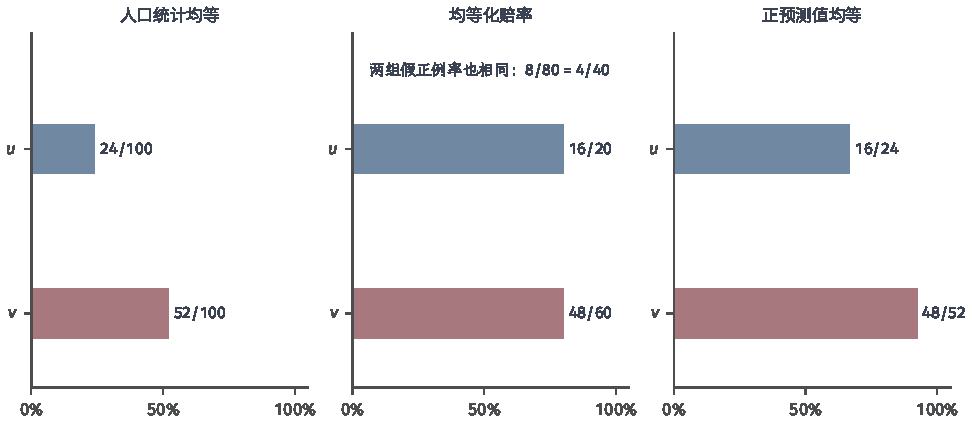
\includegraphics[width=164.600mm]{figures/03-foundations/03-trustworthiness/matplotlib/trust-fairness-incompatibility/figure.pdf}
  \caption{同一教学记录按三个分母比较：全体申请者、同资格者、已获选者。两组各100人，合格20与60，计数沿示例~\ref{ex:fairness-rates}。共同$t=0.8,f=0.1$满足均等化赔率，其他两项比例仍不同。冲突限于不同基准比例及$0<f<t<1$，$f=0$等另作分析。}
  \label{fig:trust-fairness-incompatibility}
\end{figure*}

图~\ref{fig:trust-fairness-denominators}按资格与决策交叉计数。观察分母，就能判断指标保护全体、合格者、不合格者还是获选者。

\begin{figure*}[!htb]
  \centering
  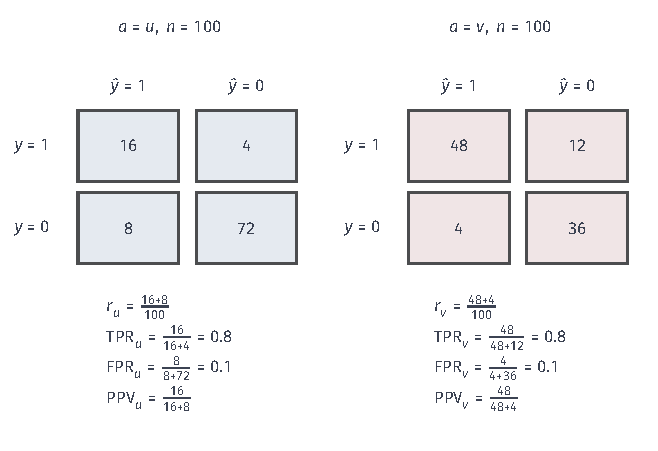
\includegraphics[width=111.404mm]{figures/03-foundations/03-trustworthiness/tikz/trust-fairness-denominators/figure.pdf}
  \caption{按资格为行、是否获选为列排列示例~\ref{ex:fairness-rates}两组计数，下方指标各取相应分母。真正例和假正例一致仍可伴随机会及预测值不同。计数未包括概率，不能检验分数校准。}
  \label{fig:trust-fairness-denominators}
\end{figure*}

混淆矩阵没有个人概率，不能检验分数。另构造两组各10人得0.8分，合格数8与6，则组内经验频率为0.8和0.6，第二组的经验频率比预测分数低0.2。这可以与前例总计数并存，说明同错误率未包括分数信息。总体校准是否失败，还要根据样本支持估计误差。

按准则保存矩阵与分数：获选除总人数、合格获选除合格人数、合格获选除获选人数，分别对应机会、真正例率和预测值。校准再按组及分数区间比较均值与频率。条件和分母不同使同一记录回答不同问题，达标对照还需第~\ref{sec:fairness-evidence}节的误差。

\paragraph{交叉群体中的分数检验}

细化组的思路也用于概率。\term{多重校准}（multicalibration）要求在可识别子群的各分数区间内，平均预测分数与实际事件频率的差不超过给定容差，Hébert-Johnson等用它限制总体校准漏掉的复杂组偏差\scite{hebertjohnson2018multicalibration}。

沿第~\ref{sec:reliability-evaluation}节分箱，先设最小概率质量下的候选$\mathcal A\subseteq\mathcal G\times\mathcal B$，$\mathcal B$为区间族。我们比较每个组区间中的平均残差，并要求全部不超容差：
\begin{equation}
 \sup_{(g,B)\in\mathcal A}
 \left|\mathbb E[y-S\mid
       g(\bm{x},a)=1,\ S\in B]\right|
 \leq\varepsilon.
 \label{eq:fairness-multicalibration}
\end{equation}
经验均值估计条件期望，全族结论要统一误差范围，搜索后只确认一个候选仍限于该候选。要求防止持续高估低估，并未要求各组成功率一致。

\subsection{相似个体的处理差异}
\label{sec:fairness-individual-comparison}

群体平均不足以保护每对相近者。\term{个体公平}（individual fairness）要求任务相关条件相近的人得到相近处理，距离及认可因素因而成为定义的一部分。

Dwork等以相似性界表达这一关系。完整审计状态$\bm z=(\bm x,a)$属于$\mathcal Z$，任务先决定哪些分量可计入距离，记录$a$不表示可据它区别待遇。令$q_{\bm z}$为决策分布、$d$为任务认可差异、$D$为决策分布差异，对全部个体对要求
\begin{equation}
 D(q_{\bm z},q_{\bm z'})\leq d(\bm z,\bm z').
 \label{eq:fairness-individual}
\end{equation}
二元规则用总变差时，$D$就是录取概率绝对差，这使“相近处理”可以量化\scite{dwork2012awareness}。

距离0.05的两人若概率0.9和0.1，违反界；若0.60和0.63，这一对达标。距离仍需规范依据，历史收入若含过去机会不平等，纳入距离可能把不平等当合理差异。结论只相对于该距离。随机化保护事前分布，同等人一次抽签仍可能结果不同。

检验先冻结距离和分布估计，搜索$D(q_{\bm z},q_{\bm z'})-d(\bm z,\bm z')>0$的个体对。如果接口直接给出决策概率，就可以计算这一超限值；如果只能重复调用随机接口，则需估计概率并给出误差区间。有限个体对中没有找到反例，只支持已检查范围内的结论，报告还应说明搜索范围和发现的最大超限值。群体准则通过，不能推出全部个体对都通过。

构造两组各一高资格一低资格，第一组只选高、第二组只选低，机会率均一半却违背同资格待遇。反过来，各组高资格比例不同而规则选全部高资格，若同资格距离0、异资格距离1，式~\eqref{eq:fairness-individual}可成立，机会率仍不同。两准则保护的关系因而互不推出。

\subsection{决策依据与影响路径}
\label{sec:fairness-counterfactual-comparison}

关注禁止因素怎样传递影响时，需要因果模型。\BookSectionRef{sec:causal-counterfactual-recourse}{第一卷“因果响应”章的“反事实与补救”一节}已建立条件反事实。反事实公平（counterfactual fairness）固定同一个体的外生背景，再比较不同群体属性干预下的预测，而非直接配对现实中的两人；Kusner等据此给出定义\scite{kusner2017counterfactual}。

令$\bm U,\bm X,A,\hat Y$为外生背景、观测、属性和预测，取值$\bm u,\bm x,a_0,b$。$\hat Y_{A\leftarrow v}(\bm U)$表示属性设为允许值$v$后的预测。对事实分布$P_{\bm X,A}$几乎处处的$(\bm{x},a_0)$，全部$b,v$满足
\begin{equation}
\begin{aligned}
 &\mathbb P\bigl(\hat Y_{A\leftarrow a_0}(\bm U)=b
       \mid\bm X=\bm x,A=a_0\bigr)\\
 &\qquad=\mathbb P\bigl(\hat Y_{A\leftarrow v}(\bm U)=b
       \mid\bm X=\bm x,A=a_0\bigr).
\end{aligned}
 \label{eq:fairness-counterfactual}
\end{equation}
事实观测先推断外生背景，同一机制再生成干预世界。只改一列却固定其后果，没有完成这种反事实传播。

构造属性$a\in\{0,1\}$、能力$u$和测验$x=u+\gamma a$，若$\gamma a$路径被认定不应影响分配，以测验$x$作为决策依据就会保留这条属性影响；在结构正确的条件下，改用$x-\gamma a=u$可以去掉该项影响。取$\gamma=2$，实际$a=1,x=7$推出$u=5$；设$a=0$后应有$x=5$，校正分数在两世界都5。保留$x=7$只改$a$没有传播结构。公平计算可能需要属性，但结构与系数不可靠时机械相减未必合理，观测分布通常不足以唯一识别它。

有些任务只禁部分路径，例如允许实际能力、禁止无关直接偏好，需要明确路径与识别条件。统一要求属性改后不变未必合适。第~\ref{sec:interpretability-recourse}节寻找个体可实施的补救行动，本节属性干预仅用于机制分析，未将属性当应改变的行动。

审计需声明图与方程，依据事实推背景，对同背景生成不同属性下决策分布，再比较式~\eqref{eq:fairness-counterfactual}。不能识别机制时，报告合理机制间的敏感性；混淆矩阵没有这种证据。计算相等也仅在因果模型成立时支持结论。

\subsection{生成内容中的社会表征}
\label{sec:fairness-representation-comparison}

培训建议还可能刻板描述、遗漏或无依据地贬低人群，录取计数无法评价这些内容。先规定表达及语境，例如证据不足时不用身份推断能力，再建立可核验标注。

受控任务固定资格、经历和请求，只改无关身份线索，比较描述、推荐、尊重及无依据断言。证据充分和不足都需测试，防止一律拒答的表面均等；文本自然性和事实含义也需核验，规则及人工复核评价输出。词替换只证明对应行为差异，未证明个体因果反事实。

随机生成需重复抽样，保存比例和波动，并在不同提示检查稳定性。评分者也可能产生偏差，因此需要用已核实标签的样本检查评分与这些标签是否一致，并分析常见误判；多人评分时，还应报告评分者之间的一致程度。BBQ区分模糊和非模糊语境，提示内容评价需保留证据充分性及文化、语言范围\scite{parrish2022bbq}。

\subsection{公平要求的声明}
\label{sec:fairness-requirements}

要将上述证据用于判定，先写任务、人群、保护关系、资格标准、禁止路径与优先后果，再定主要准则、容差、效用和资源限制，说明验证数据与期限。指标名称只给一种测量，尚未形成完整公平要求。

要求还需责任依据。识别法律、政策与领域义务，保存受影响者、专家、运行方的意见及分歧，明确由谁批准准则、容差、最低水平、资源安排及属性用途。批准理由、未解决异议、纠正入口和复查周期应可追溯。这些程序不能消除价值冲突，但可以帮助区分机构偏好、观测到的比例与已经获得认可的规范依据。

教学系统可取独立资格为$y$，预设两个群体真正例率绝对差不超0.05、两组都至少0.8，名额受预算约束，并报告假正例、交叉组和申请成本。数值是构造标准。差距约束限制两组之间的差异，最低水平要求则保护各组的合格者获选率。若仍有一组低于下限，只降低另一组的获选率并不能达标。资源与要求冲突，应重新讨论而非隐藏条件。

属性用途也进入声明。训练与审计用$a$构造约束，不直接决定部署能否读取；后者由责任流程规定。分组阈值必须识别组别，训练约束却可能得到无需属性的预测器，允许用途决定候选方法。

意图与结果分开记录：目标说明打算满足什么，验收说明哪个版本在何人群、数据和假设下有何证据。独立检验未完、组样本不足或因果不可识别时保留限制，去偏算法名称无法证明公平。

\subsection{判定结论的形成}
\label{sec:fairness-compatibility}

五类证据分别对应要求，综合判定还需说明本次选择哪些准则、能否兼容、样本及假设支持到哪里。某分支通过只给局部结论，不能直接合成无条件“系统公平”。

\paragraph{准则之间的取舍}

同一系统承担的准则可能相互冲突，指标分歧未必来自训练不够。下面由群体比例推导兼容条件，限定共同可选择的目标，而非增加一种审计方法。

例~\ref{ex:fairness-rates}中，相同错误率仍产生不同机会。设正例比例$\pi_a$、真正例率$t_a$和假正例率$f_a$，按资格分解机会率得到
\[
 r_a=\pi_a t_a+(1-\pi_a)f_a.
\]
若共用$t,f$且$t\ne f$，不同$\pi_a$就给不同$r_a$。在上述条件下再要求$r_a$相同，就无法同时保持这两个共同错误率。

同样条件还决定获选者的资格。若共同真正例$t$、假正例$f$，各组$\pi_a\in(0,1)$且正决策概率大于零，Bayes公式给出
\begin{equation}
 \mathbb P(y=1\mid\hat y=1,a)
 =\frac{t\pi_a}{t\pi_a+f(1-\pi_a)}.
 \label{eq:fairness-predictive-value}
\end{equation}
$t,f>0$时右侧随$\pi_a$严格增加，基准比例不同就无法同时共用正预测值。结论不依赖分类算法，却需保留边界：$f=0$时预测值可能都1。更一般的分数公平取舍也应连同条件理解\scite{kleinberg2016fairness}。

另一项冲突涉及分数。令部署$S\in[0,1]$组内校准，且各组$0<\pi_a<1$，记正负例平均$\mu_{1,a}=\mathbb E[S\mid y=1,a]$、$\mu_{0,a}=\mathbb E[S\mid y=0,a]$。若分别跨组共用$\mu_1,\mu_0$，全期望给出
\[
 \pi_a=\mathbb E[S\mid a]
       =\pi_a\mu_1+(1-\pi_a)\mu_0.
\]
不同基准比例两式相减得到$\mu_1-\mu_0=1$，有界分数迫使$\mu_1=1,\mu_0=0$，即完美预测。因此非完美分数、不同基准比例下三项不能共存。平均分数平衡不是式~\eqref{eq:fairness-equalized-odds}的二元率平衡，条件不可混用。

冲突需要依据已记录规范和参与过程设优先级。例如优先避免误拒合格者，可用机会均等为主约束，同时公开假正例、名额与预测值的代价。没有优化的准则仍需报告，移出目标不等于其后果消失。

\paragraph{有限样本与建模假设}
\label{sec:fairness-evidence}

准则规定总体关系，有限数据只提供估计。群体受样本与分母限制，个体另受距离限制，反事实另受机制限制；后两项不会因更多样本自动正确。我们分别报告假设敏感性和抽样误差，再以群体差说明判定。

真正例分母是组内正例，假正例分母是组内负例，小交叉组可能缺证据，多组搜索也增加偶然极值。敏感属性若经补全，其估计误差同样进入审计，不能视作无误身份。

先在审计标签揭示前冻结模型、阈值、指标、容差和两组。审计数据不参与这些选择，各组正例分别独立同分布地来自目标人群的组内正例分布，其数量为$n_u,n_v$，真正例率的估计记为$\hat t_u,\hat t_v$。预设$\delta\in(0,1)$，分别使用Hoeffding并联合控制，以至少$1-\delta$有
\[
 |(t_u-t_v)-(\hat t_u-\hat t_v)|
 \leq
 \sqrt{\frac{\log(4/\delta)}{2n_u}}
 +\sqrt{\frac{\log(4/\delta)}{2n_v}}.
\]
一组正例少便使差距界宽，总样本多不能补偿。要求$|t_u-t_v|\leq\eta$时，需将经验绝对差加上误差界后仍不超$\eta$；未拒绝零差不能证明差小。资料参与选模、调阈值、挑指标或搜索后，需独立审计或候选统一界，不能保留单次解释。

\paragraph{达标、违反与证据不足}

相对容差，可靠上界仍在界内支持达标，下界已超界支持违反，范围跨界则证据不足。个体另给距离与搜索，因果另给机制，内容另给任务及评分。未发现违规或统计不显著，均不足以单独宣称公平。

报告保留各组水平、准则、数据和版本，同时指出未覆盖人群及假设。这才确定了干预要补的要求与情境，选择补采、重训或流程调整还要看形成原因。

\section{公平性的干预}
\label{sec:fairness-intervention}

相同机会差可能由数据遗漏、资格标签、训练加权或决策规则产生。判定提供未满足的要求，机制提供修改位置，两者结合才能选择干预；差距本身没有指定某个算法。

下面按数据、训练和服务三个位置处理已声明要求。补充与核实数据、调整学习规则、改变把分数转成行动的规则，可以组合使用，但解决的问题不同。例如，补充少数群体的数据后，仍可能需要调整训练中的错误代价；训练约束通过后，也仍需检查申诉过程的等待时间。最后用即时与长期证据决定措施是否改善处境。

图~\ref{fig:trust-fairness-intervention-stages}沿数据、训练和决策画出干预位置。发生在其他位置的问题未必能由当前环节的指标调整修复，因此还要沿完整后果验收。

\begin{figure*}[htbp]
  \centering
  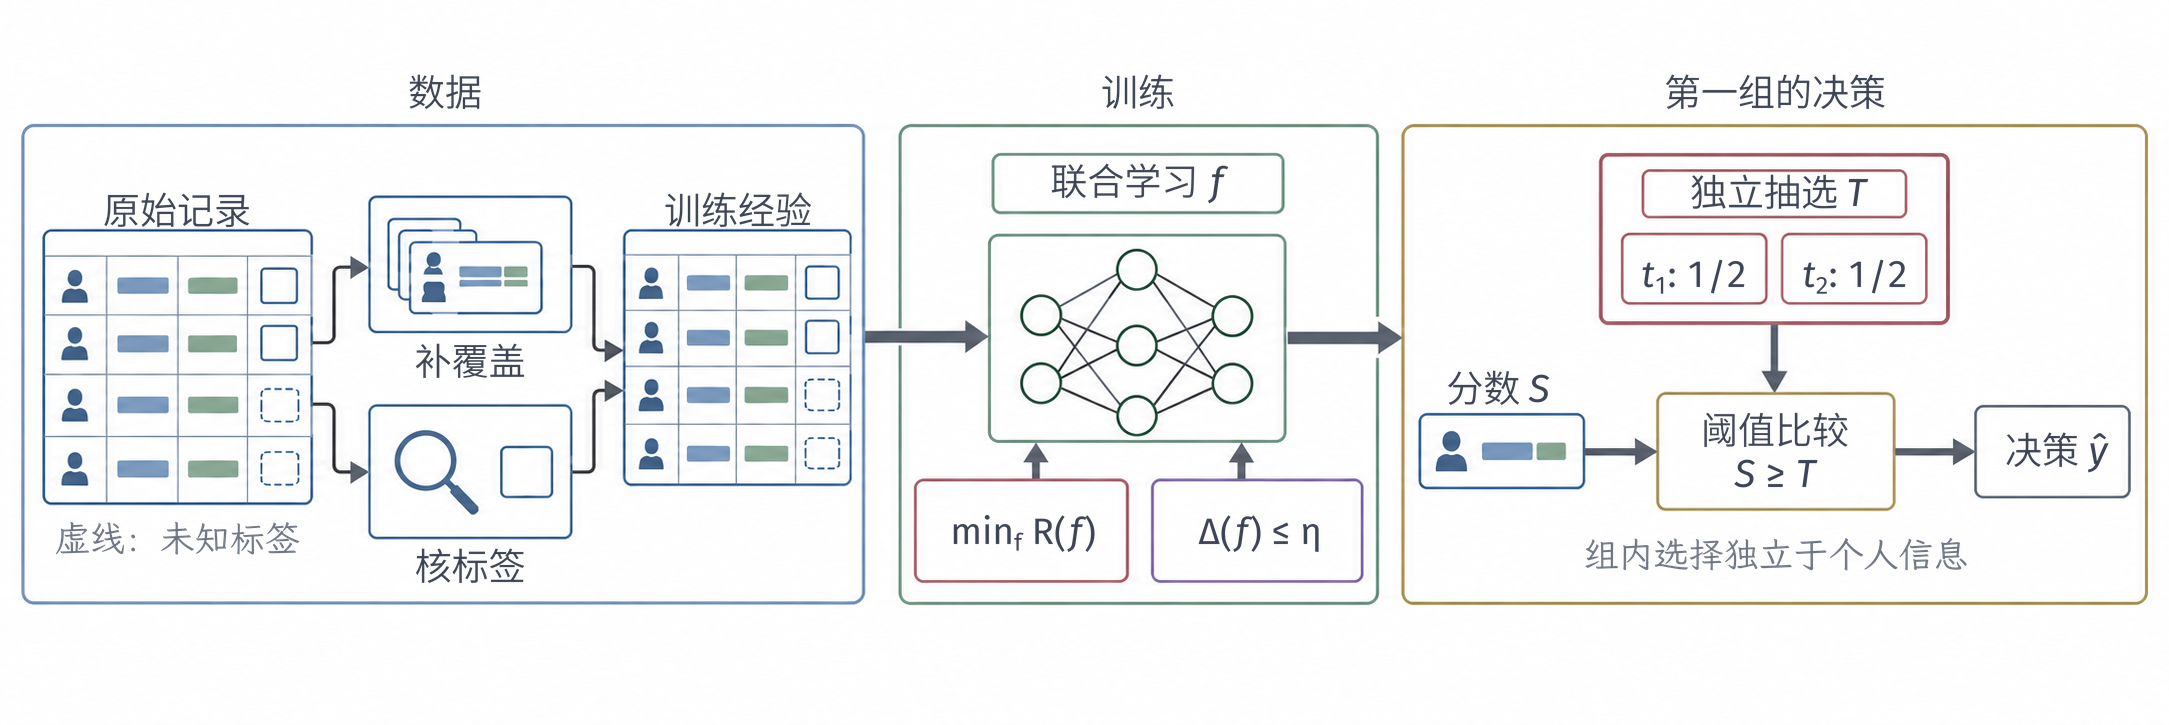
\includegraphics[width=164.600mm]{figures/03-foundations/03-trustworthiness/generated/fairness-interventions/figure.png}
  \caption{数据环节补充遗漏人群并核实标签，训练环节调整风险目标及公平约束，决策环节采用随机化阈值；三个位置的措施可以组合。虚线记录标签未知，$\hat y$为决策。每组以固定各半概率选两个阈值，选择独立于个人分数、特征及真值，数值见示例~\ref{ex:fairness-random-threshold}。单环节达标未保证系统全部要求。}
  \label{fig:trust-fairness-intervention-stages}
\end{figure*}

\subsection{数据采集与质量的改进}
\label{sec:fairness-data-intervention}

遗漏人群时，按任务、条件与交叉组定位缺少的语言、设备、地区或资格区间，再扩采集渠道。新增多少有效观测要对应之前哪个缺口，人数相同不是充分目标。重复旧样本只能改变训练频率，未增加独立个体信息。

训练可有意多采困难群体，评价则说明代表目标人口还是平衡审计人口。改比例会改变平均含义，分组结果仍须保留，必要时按有依据目标权重汇总。新审计资料独立于干预选择，才能避免反复调试后的选择偏差。

测量问题要核查同字段跨组含义，用语言、设备配对及可靠参照区分真实与测量差。标签问题要复核资格、指南和争议，必要时重标。修正错误或不合理目标须保留依据，不能为比例相同改写真实结果。

结果缺失不能填作失败。培训只观察获选者时，寻找独立资格测验、调查或其他可靠观测；改变选择取得证据要说明实施条件，统计修正则需概率和识别条件，见第~\ref{sec:fairness-long-term}节。更多获选记录未自动增加被拒者信息。

采集、测量与标签改变需随数据留痕。数据集说明书的用途、组成、采集和范围帮助定位人群遗漏和误用，记录却未替代实际补采及核验\scite{gebru2021datasheets}。

改好数据仍未决定分配原则。训练若继续用多数收益抵消小组损失，需要改学习规则；分数转行动仍有问题，则转到服务流程检查。

\subsection{训练目标与学习规则的调整}
\label{sec:fairness-learning-intervention}

已有依据被模型不合理使用时，可改样本错误代价、约束表示信息或直接约束公平指标。三者都在训练中起作用，但分别改变样本对损失的贡献、表示保留的信息，以及学习器对公平准则违反程度的响应，需要按形成原因选择。

令训练数据$\mathcal D_{\mathrm{tr}}$、候选$\mathcal F$确定经验风险$\widehat R_{\mathrm{tr}}(f)$和选定差异$\widehat\Delta_{\mathrm{tr}}(f)$。先在差异容限$\eta$内比较风险，得到
\[
\begin{aligned}
 \min_{f\in\mathcal F}\quad &\widehat R_{\mathrm{tr}}(f)\\
 \text{subject to}\quad &\widehat\Delta_{\mathrm{tr}}(f)\leq\eta.
\end{aligned}
\]
目标总体的$R(f),\Delta(f)$需独立审计。惩罚$\widehat R_{\mathrm{tr}}+\lambda\widehat\Delta_{\mathrm{tr}}$、$\lambda\geq0$便于求解，固定系数仍未证明约束满足。

图~\ref{fig:trust-fairness-pareto}在构造200人资料中同时比较准确率与真正例率绝对差。准确率不低、差距不大且至少一项严格改善时，候选支配另一候选；当前未被支配者形成有限帕累托集合（Pareto set）。换候选、指标或评价资料会改变这个集合，不能看作普遍边界。

\begin{figure}[htbp]
  \centering
  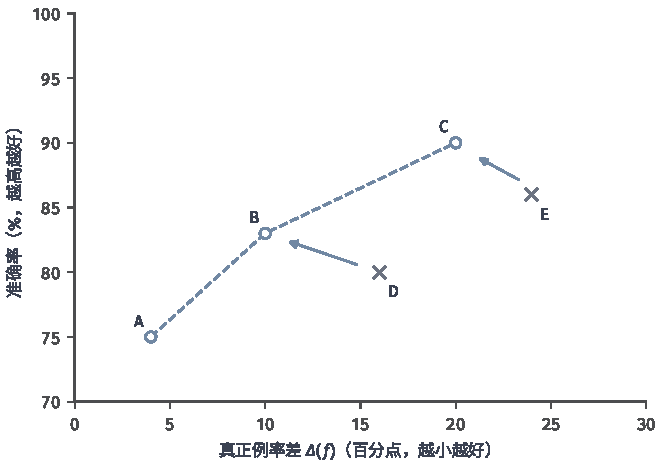
\includegraphics[width=\linewidth]{figures/03-foundations/03-trustworthiness/matplotlib/trust-fairness-pareto/figure.pdf}
  \caption{构造两组各100人、各50人合格，由五套混淆计数得到“真正例率绝对差、准确率”。A、B、C为（4个百分点，75\%）、（10个百分点，83\%）、（20个百分点，90\%），D、E为（16个百分点，80\%）、（24个百分点，86\%）。B支配D、C支配E，空心圆是当前候选中的不可支配者。虚线引导阅读，未证明中间点可实现。}
  \label{fig:trust-fairness-pareto}
\end{figure}

\paragraph{不同样本与错误的训练代价}

为让两组各占经验损失一半，训练人数$n_u,n_v>0$、总$n=n_u+n_v$时，可给组$a$每样本权重$\omega_a=n/(2n_a)$，得到
\[
 \frac1n\sum_{i=1}^{n}\omega_{a_i}\ell(f(\bm x_i),y_i)
 =\frac12\hat R_u(f)+\frac12\hat R_v(f),
\]
$\hat R_a$为组内损失。训练梯度按权重累积，之后独立检查公平量。小组不再仅因少而被忽略，但错误率未被强制相同，标签也未被修复；半半目标仍需任务批准。

\paragraph{表示中的信息依赖}

多个任务复用特征时，可以在表示中限制群体信息。Zemel等的Learning Fair Representations将样本软分配到原型，同时比较重构、预测和组间原型分配。它约束变换后的编码，不只是删字段\scite{zemel2013fairrepresentations}。

记原型概率$q_k(\bm{x})$，组均值$\bar q_{k,a}$，可用$\sum_k|\bar q_{k,u}-\bar q_{k,v}|$惩罚。若先按$q_k$抽原型，再只依原型决策，各组平均分配完全相同便由全概率得相同机会。经验近似相同或把整个软向量交任意预测器，没有这一无条件继承；下游用法改变需重新检验。

训练共同调整原型、分配和预测器。重构防止丢全部信息，预测保留任务区分，分配惩罚减少指定差别，权重控制取舍。独立资料还要分别测效用、群体可预测性和最终决策，仅惩罚下降未证明下游公平。

也可以训练一个辅助预测器寻找残留信息。\term{对抗去偏}（adversarial debiasing）使任务模型与根据表示或输出猜属性的对手竞争。Zhang等将其用于减少特定差距，效果仍取决于对手所见与能力\scite{zhang2018debiasing}。

令任务输出$h_{\bm{\theta}}$、属性预测器$d_{\bm{\phi}}$，经验任务和群体损失为$L_{\mathrm{task}},L_{\mathrm{group}}$，取舍系数$\lambda\geq0$。竞争目标可写为
\[
 \min_{\bm{\theta}}\max_{\bm{\phi}}
 \left\{L_{\mathrm{task}}(\bm{\theta})
       -\lambda L_{\mathrm{group}}(\bm{\theta},\bm{\phi})\right\}.
\]
固定任务模型时训练对手降低群体损失，固定对手时降低任务损失、提高群体损失，部署通常只留任务模型。另训独立攻击者检查是否绕过原对手。只看输出时，这减少的是给定函数类、样本和优化精度可检测依赖；均等化赔率需控制标签内剩余依赖，可分标签训练。对手未胜基准没有证明独立或排除更强者；竞争不稳、任务与属性信息重叠仍会产生取舍。

\paragraph{公平约束下的分类学习}

表示约束间接改变公平，已知准则也可直接转为条件矩，即指定群体和标签中预测指示或损失的平均。例如真正例率差拆为$\hat t_u-\hat t_v\leq\eta$及逆向一项，各$\hat t_a$由组正例的指示均值得到。Agarwal等把外层公平约束归约为\term{成本敏感分类}（cost-sensitive classification），调整每样本每种错误代价，再调用既有学习器，保留其表示形式\scite{agarwal2018fairreductions}。

记候选$\mathcal F$、有限约束$\mathcal J$，带方向的经验差异$\hat g_j(f)$与容限$\eta_j$，超限量为$\hat g_j(f)-\eta_j$，约束对随机分类器混合线性。部署按支持于$\mathcal F$的分布$Q$抽规则，拉格朗日形式为
\begin{equation}
\begin{aligned}
 &\min_{\substack{Q:\ \operatorname{supp}(Q)\subseteq\mathcal F}}
 \sup_{\bm{\lambda}\in\mathbb R_+^{|\mathcal J|}}
 \left\{\mathbb E_{f\sim Q}[\widehat R_{\mathrm{tr}}(f)]\right.\\
 &\qquad\left.+
 \sum_{j\in\mathcal J}\lambda_j
 \bigl(\mathbb E_{f\sim Q}[\hat g_j(f)]-\eta_j\bigr)
 \right\}.
\end{aligned}
 \label{eq:fairness-reduction}
\end{equation}
乘子可取任意非负值，因此只要某项平均差异超过容限，就能不断增大该项乘子，使上确界变为无穷大；满足全部约束的混合才保留有限的风险值。训练时，乘子为违反准则的错误增加成本，学习器响应这些成本。多轮分类器的混合还可产生单一确定规则无法实现的中间率。实际算法另限制乘子域和停止精度，公式只说明约束作用。

若某组真正例率低于要求，就增加该组正例被误拒的代价；若调整后假正例率超过上限，则提高该组负例被误收的代价，抑制过多的错误录取。反馈可追踪到哪组哪种错误，未将“惩罚越大”当作充分改进。

从初始乘子训练、计算违规、增大违规项乘子并重复，保存候选及最终混合权重，不能只选准确率最高的一轮。此法直接反馈准则，对抗去偏反馈可预测属性；优化形式相似没有使两者同义。

归约依赖候选族、成本学习器能力和求解误差，经验达标仍需独立总体审计及容差。属性可仅在训练构造约束，部署读取什么由模型族决定，与使用时必须识组的后处理不同。

交叉组太多时，可交替学习与审计：搜索当前最高加权违规组，将相同参照、质量和差异转为下一轮约束。改一交叠组可能影响其他组，停止要检查约定全族并独立验证，不能只看最后发现的组。

个体要求可按认可距离惩罚决策差超限，再用未优化个体对检验；反事实要求可按认可因果结构构造不受禁路径的依据或约束世界间一致。测验$x-\gamma a$仅在结构成立时有效，优化一致没有修复不可靠机制。总体比例均等不能代替这两项。

\subsection{决策规则与服务流程的调整}
\label{sec:fairness-decision-intervention}

无法重新训练模型时，仍可修改两种对象：分数失准时调整分数；机会分配或错误率违反要求时，调整把分数转成行动的规则。二者会互相影响，各自达标仍需分别检验。

针对式~\eqref{eq:fairness-multicalibration}，可按组区间平均残差修分数，再检查交叠组；正式方法还控制步长、搜索和泛化。新分数要重新校准，下游固定阈值的获选名单也可能改变，所以分配量须重算。

保留原分数而改规则，可选择组别阈值，每组形成ROC中的假正例、真正例点。以预设概率为每人独立于分数、其他特征和标签选两个阈值，期望率才是点的凸组合。Hardt等据可达区域选择满足均等化赔率的共同错误点。

\begin{example}[随机化如何补出共同错误率]
\label{ex:fairness-random-threshold}
构造独立验证结果：第一组两阈值的$(f,t)$为$(0.1,0.5)$、$(0.3,0.9)$，第二组一阈值为$(0.2,0.7)$。第一组每人按预设各半概率独立选阈值，且独立于分数、其他特征与标签，平均点便为$(0.2,0.7)$。两组在这批验证记录上的期望错误率相同，一次实际随机选择得到的样本率仍可能波动。部署时还要检查目标分布是否支持这些率，并估计相应误差。
\end{example}

共同可达点的真正例率可能低于下限，假正例率可能超过上限，效用也可能低于要求。错误率均等有时是通过降低原本较好组的获选水平实现的。后处理不能增加原排序信息，也可能给相近个体因组别而不同机会，未保证个体公平。其收益是固定分数下可算取舍，限制是表示和排序固定。采用须符合属性用途、资源与实际后果。

服务干预还包括复核、补材料、纠错以及语言和提交渠道支持，需记录标准与时延。人工不是公平证明，要分别检查各组转交、等待和最终结果；大量转人工却迟迟不服务，自动错误减少也未证明改善。

生成建议可在服务规则中限定证据、请求信息和复核表达，再用受控身份任务验收。训练也可用核实对照及反馈，“用了去偏数据”仍不是内容达标证据。

\subsection{干预效果与持续调整}
\label{sec:fairness-intervention-evaluation}
\label{sec:fairness-long-term}

各位置干预都返回同一要求验收。即时比较评估当下收益，长期跟踪检查数据和状态改变后是否仍满足要求，结合结果决定保留、调整或撤回。

\paragraph{即时效果与负担转移}

即时对照固定任务、群体、标签和准则，在未用于选择的同一批资料比较规则，保存效用、组指标、目标及变化误差。若过程改变人群和标签，还需后续识别。例如，两组真正例率的差距从0.2降为零，既可能是原本较低的一组从0.6升到0.8，也可能是原本较高的一组从0.8降到0.6。只有同时记录修改前后的真正例率、假正例率和获选名额，才能判断合格者机会是否改善；还需检查负担有没有转移给其他人或其他环节。

模型暂不作出自动决定而将请求转交人工时，需按组报告第~\ref{sec:reliability-evaluation}节的处理比例及接受风险。大量转交某组的请求，可能降低自动处理部分的错误率，却未证明服务更公平，等待、人工成本和结果仍要计入。服务覆盖指获得处理比例，与集合覆盖真实标签不同。

主要标准先由要求确定，其他指标揭示代价；不断挑最有利指标会只显示局部收益。样本不足时报告不确定，差异不显著未证明不公平消失。

\paragraph{选择性标签与后续结果}

长期干预改变比较条件本身。曝光增加会产生更多点击证据，培训又改变未来能力和资格。静态通过之后，仍要追踪机会、能力与负担的动态。

如果给定特征与群体属性后，获选与培训后的潜在结果没有额外关联，且各类人都有正的获选概率，就可以尝试按选择概率加权，修正结果只对获选者可见所造成的偏差。这些条件分别称为条件可交换性与正概率覆盖，下一段将写出它们的数学形式。某类从未获选时，没有正概率就无法恢复其结果，需要另取得证据并核查取得条件。

Lakkaraju等利用不同决策者的选择差异研究选择性标签评价，说明验证标签可能由待评价决策产生。决策者差异仍需比较假设，不能直接认作随机实验\scite{lakkaraju2017selective}。

为避免把后续收益混入资格，记培训结果$z$，获得机会$r=1$，潜在结果$z(1)$，选择概率$e(\bm{x},a)=\mathbb P(r=1\mid\bm{x},a)$。若给定特征和属性时$r$独立于$z(1)$，目标中$e>0$且获选者$z=z(1)$，逆概率加权给出
\begin{equation}
 \mathbb E\!\left[\frac{r z}{e(\bm{x},a)}\mid a\right]
 =\mathbb E[z(1)\mid a].
 \label{eq:fairness-selective-weight}
\end{equation}
$r=0$时乘积定义零，无需观察其$z$。先条件化再用独立性消去选择概率，最后组内平均便得右侧。审核者使用未记录的信息，可能破坏这一条件独立性，小概率放大方差，做加权之前需检查这些条件。

Liu等的Delayed Impact of Fair Machine Learning进一步用决策后状态模型分析，静态约束在其假设下可帮助也可损害保护组。方向由新增获选者、状态变化机制和原分布共同决定\scite{liu2018delayedimpact}。

构造获得机会后成功使状态增加1、失败使状态减少2的情形，成功概率为$p$，期望净变为$p-2(1-p)=3p-2$。$p=0.5$时每个新增参与者平均减0.5，所以机会增加未必改善状态。这是机制例而非培训数据；在其他人的状态保持不变的这个模型中，新增正决策的条件净收益为正，才会提升群体的平均状态，每人改善还需更强条件。费用补助、课程改变或失败代价降低，也可改变结果。

新差异出现后，回到数据、测量和干预副作用定位原因，再用声明标准与新证据调整；继续增加当前差距惩罚未必改对机制。

\Needspace{8\baselineskip}
\section{本章小结}
\label{sec:fairness-summary}

培训分配要先给差异的规范依据，再分别检查机会与负担、预测错误与分数含义、个体待遇、影响路径和社会表征。统计、距离、因果与内容证据各有条件，准则又可能冲突，结论应限定任务、人群及证据，区分达标、违反和不足。

没有满足要求时，应按形成原因补充遗漏人群的数据、修正测量与标签、调整训练或改变服务流程。这些措施可以组合，却不能互相替代。验收时保存各组原有水平、实际收益及后续变化，避免通过降低服务水平或转移负担得到表面的比例一致。某指标改善仍可能没有实现本意，下一章将扩到一般目标与行为边界；采集审计所需属性也受第~\ref{chap:trust-privacy}章的信息保护限制。

\paragraph{延伸阅读}

机会均等后处理与个体公平分别保护标签条件率和任务相似性，对照Hardt等与Dwork等可辨认各自对象、冲突及不互推关系\scite{hardt2016opportunity,dwork2012awareness}。

反事实公平与延迟影响分别依赖因果机制和后续状态模型，Kusner等与Liu等的分析可帮助区分经验率、允许路径与长期后果；结论都需保留建模假设\scite{kusner2017counterfactual,liu2018delayedimpact}。
